\chapter{MARCO METODOLÓGICO}

En este capítulo se describe de manera detallada la metodología empleada para
diseñar, implementar y evaluar un sistema robótico teleoperado con
retroalimentación háptica, orientado a mejorar la precisión y seguridad en
procedimientos de sutura en heridas superficiales. La ruta metodológica sigue
un enfoque experimental, en el que se desarrollan y validan componentes
mediante simulaciones en entornos que toman en consideración variables físicas
como la masa, gravedad e inercia y análisis cuantitativos que aseguren la
viabilidad técnica del sistema acorde a los parámetros de desempeño del
controlador para el seguimiento de la trayectoria.

\section{Metodología de desarrollo basada en la norma VDI 2206}

El desarrollo del sistema robótico se estructuró siguiendo la norma VDI 2206,
una metodología reconocida para el diseño de sistemas mecatrónicos que propone
un enfoque en “V” modificado. Esta metodología permite una integración temprana
y concurrente de los dominios mecánico, electrónico y de control, promoviendo
la validación continua desde las etapas iniciales del diseño.

La metodología contempla una fase exploratoria, donde se analizan los
principios físicos, conceptos funcionales y alternativas tecnológicas, y una
fase sistemática de diseño, donde se desarrollan modelos del sistema,
simulaciones, implementación física y validación final.

En este proyecto, la fase exploratoria incluyó el análisis de los
requerimientos del procedimiento de sutura, la evaluación de dispositivos
candidatos (UR5, Geomagic Touch) y la definición preliminar de principios
físicos relevantes (fuerzas de interacción, precisión posicional, escalamiento
de movimientos). Posteriormente, en la fase de desarrollo sistemático, se
aplicó la metodología en cuatro etapas clave:

\begin{enumerate}
    \item Diseño conceptual: definición de arquitectura del sistema,
          identificación de comunicación entre componentes y especificaciones
          funcionales.
    \item Modelado y simulación: desarrollo del modelo dinámico del UR5 y
          simulación del entorno en Gazebo con los elementos 3D añadidos.
    \item Implementación: integración de nodos ROS 2, C++, librerías oficiales
          de los equipos utilizados y protocolos de comunicación entre estos.
    \item Validación: pruebas en escenarios reales en el laboratorio de
          Ingeniería Mecatrónica para medir precisión, respuesta dinámica y
          calidad de la
          retroalimentación háptica.
\end{enumerate}

\begin{figure}[H]
    \centering
    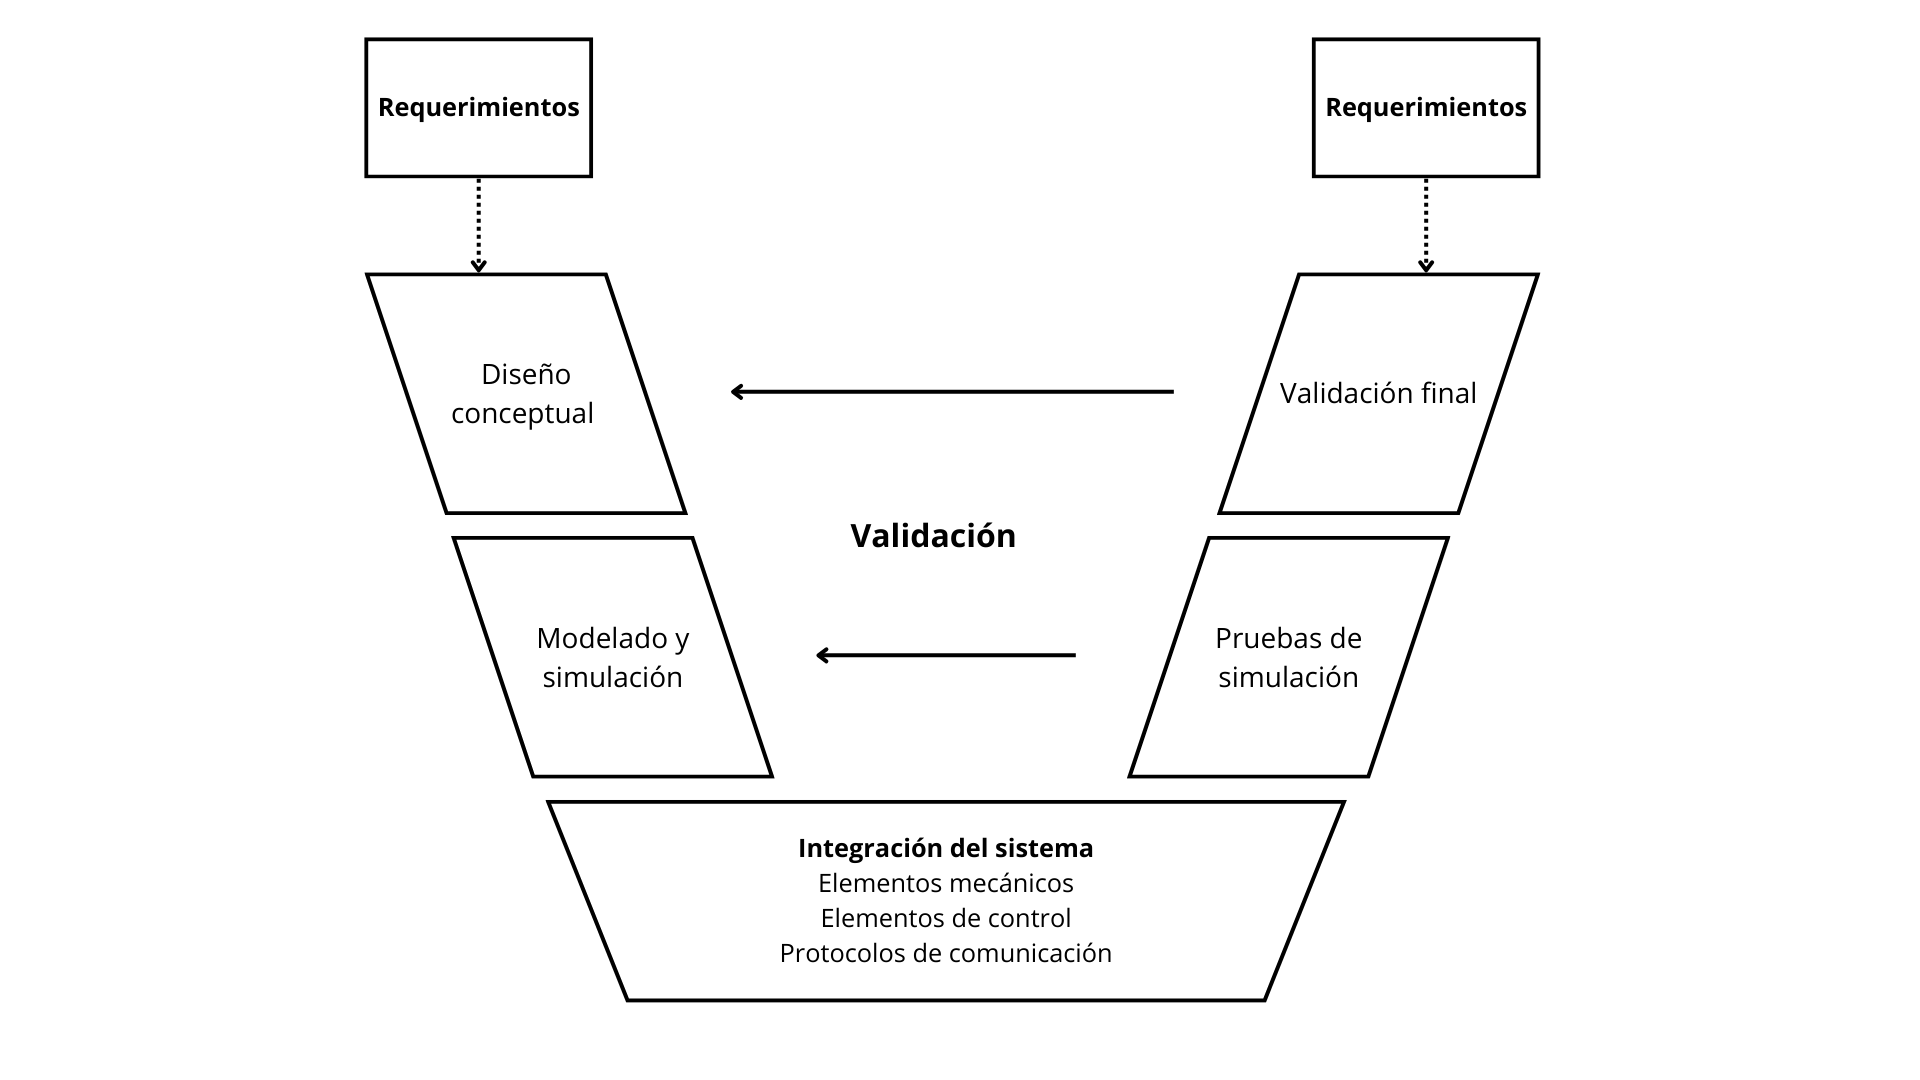
\includegraphics[width=1\linewidth]{images/vdi_muy_basico.png}
    \caption{Esquema de la metodología VDI 2206}
    \label{fig:enter-label}
\end{figure}

\section{Diseño del sistema robótico}

En esta fase inicial se establecen los requerimientos funcionales y técnicos
del sistema robótico, considerando las demandas propias del procedimiento de
sutura. Se seleccionan los dispositivos principales, incluyendo el manipulador
UR5 y el dispositivo háptico Geomagic Touch, definiendo sus roles dentro del
sistema. Además, se desarrolló un modelo cinemático y dinámico del UR5
utilizando el método de Denavit-Hartenberg, lo que permitió determinar la
posición en tiempo real del efector final con base en los valores articulares y
facilitar su integración en la plataforma de simulación.
\begin{table}[H]
    \begin{center}
        \begin{tabular}{| c | c | c | c | c |}
            \hline
            i & $d_i$    & $\theta_i$  & $a_i$    & $\alpha_i$       \\ \hline
            1 & $0.1625$ & $q_1$       & $0$      & $-\frac{\pi}{2}$ \\ \hline
            2 & $0$      & $q_2$       & $0.425$  & $0$              \\ \hline
            3 & $0$      & $q_3$       & $0.3922$ & $0$              \\ \hline
            4 & $0.1333$ & $q_4 - \pi$ & $0$      & $\frac{\pi}{2}$  \\ \hline
            5 & $0.0997$ & $q_5+\pi$   & $0$      & $\frac{\pi}{2}$  \\ \hline
            6 & $0.0996$ & $q_6$       & $0$      & $0$              \\ \hline
        \end{tabular}
        \caption{Tabla de parámetros Denavit-Hartenberg}
        \label{tab:DH}

    \end{center}

\end{table}
En paralelo, se configuró un entorno virtual en Gazebo v11, utilizando ROS 2
Humble como marco de trabajo. Al poder simular las condiciones físicas reales,
como la gravedad, y las interacciones con objetos simulados, se logró realizar
pruebas preliminares en un contexto controlado y seguro.

\begin{figure}[H]
    \centering
    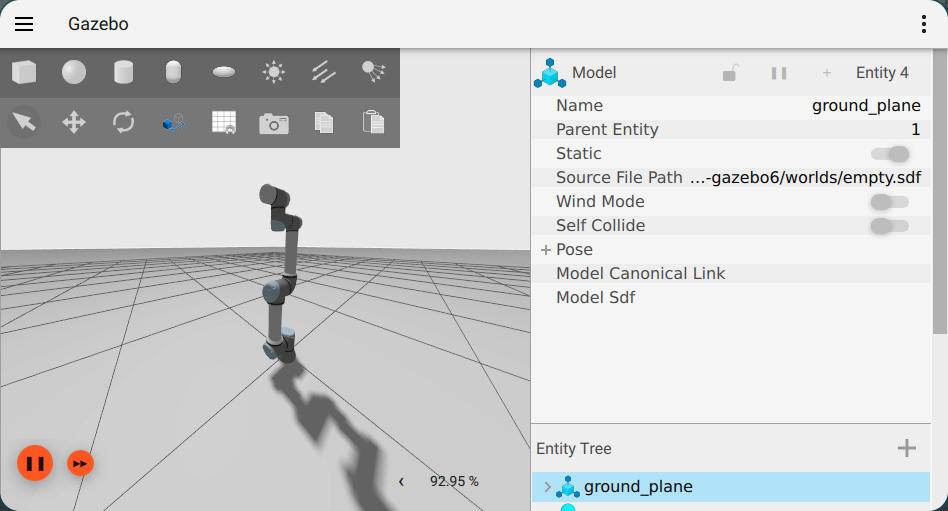
\includegraphics[width=0.75\linewidth]{images/gazebo.png}
    \caption{Entorno de Gazebo con el Robot UR5e}
    \label{fig:placeholder}
\end{figure}

\begin{figure}[H]
    \centering
    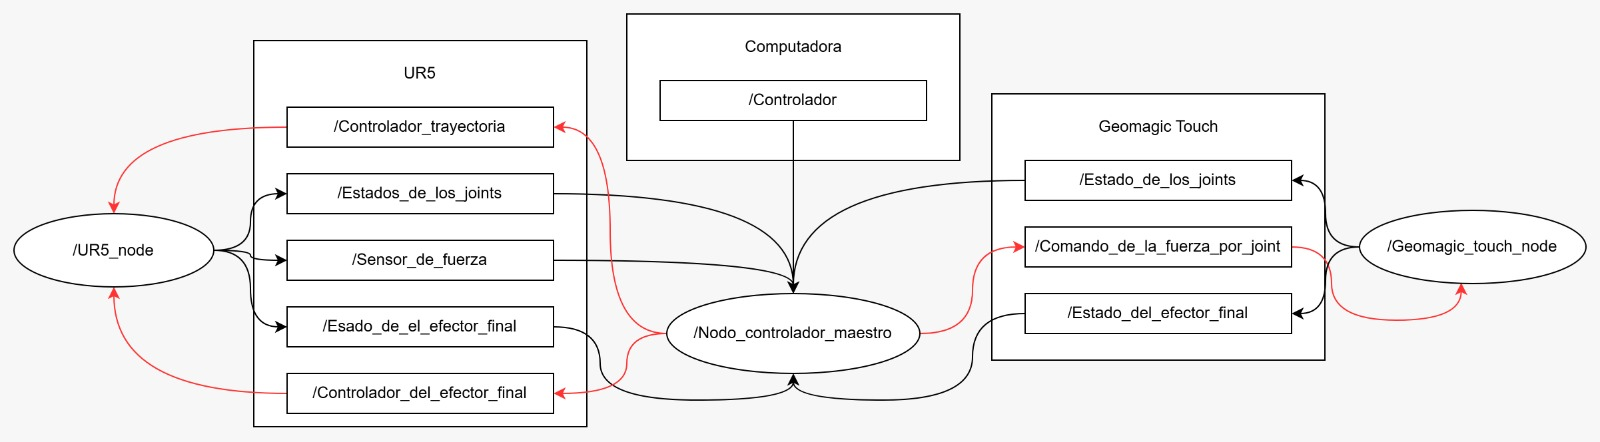
\includegraphics[width=1\linewidth]{images/comunication_desired.png}
    \caption{Comunicación de tópicos y nodos planteada}
    \label{fig:enter-label}
\end{figure}

\section{Implementación del sistema de control}

El desarrollo del control se centra en dos dispositivos clave: el manipulador
UR5 y el Geomagic Touch. Para el UR5, se diseñaron tanto un controlador basado
en dinámica inversa como un optimizador cinemático, ambos permiten generar
movimientos precisos en función de las entradas de posición y velocidad
admitidas por el fabricante. Estos controladores se complementan con un módulo
de optimización, propio del fabricante, para ajustar los parámetros de
desempeño, logrando un balance adecuado entre velocidad de respuesta y
precisión.

En el caso del dispositivo háptico, se calibra su capacidad para enviar y
recibir señales de posición y fuerza, estableciendo un puente efectivo entre el
usuario y el manipulador robótico. Además, se desarrollan transformaciones que
escalan los movimientos del dispositivo háptico al espacio de trabajo del UR5,
garantizando que las acciones del operador se reflejen fielmente en la
teleoperación.

\subsection{Interfaz háptica-robótica}

Para enlazar el sistema háptico, se utiliza el software que brinda la empresa
3D Systems para el sistema operativo Linux. Este software de OpenHaptics
permite desarrollar el controlador en C/C++. De esta forma, dado que los robots
manipuladores también se controlan en este sistema operativo, el intercambio de
información se realiza mediante la publicación y suscripción de nodos en ROS.
Además, teniendo en cuenta que el robot manipulador es teleoperado, se controla
principalmente la parte del efector final con la punta del lápiz que porta el
dispositivo háptico, ya que la forma del controlador y la del brazo no son
similares; sin embargo, se busca que ambos lleguen a tener posiciones similares
para que el movimiento sea más fluido. Asimismo, se implementa una interfaz
gráfica donde se puede observar el movimiento del robot en tiempo real con
Rviz. Estas tareas son similares a las descritas en
\cite{teleoperation_irb120_geomagic}, donde se realizó un proceso similar para
un robot ABB IRB 120.

\begin{figure}[H]
    \centering
    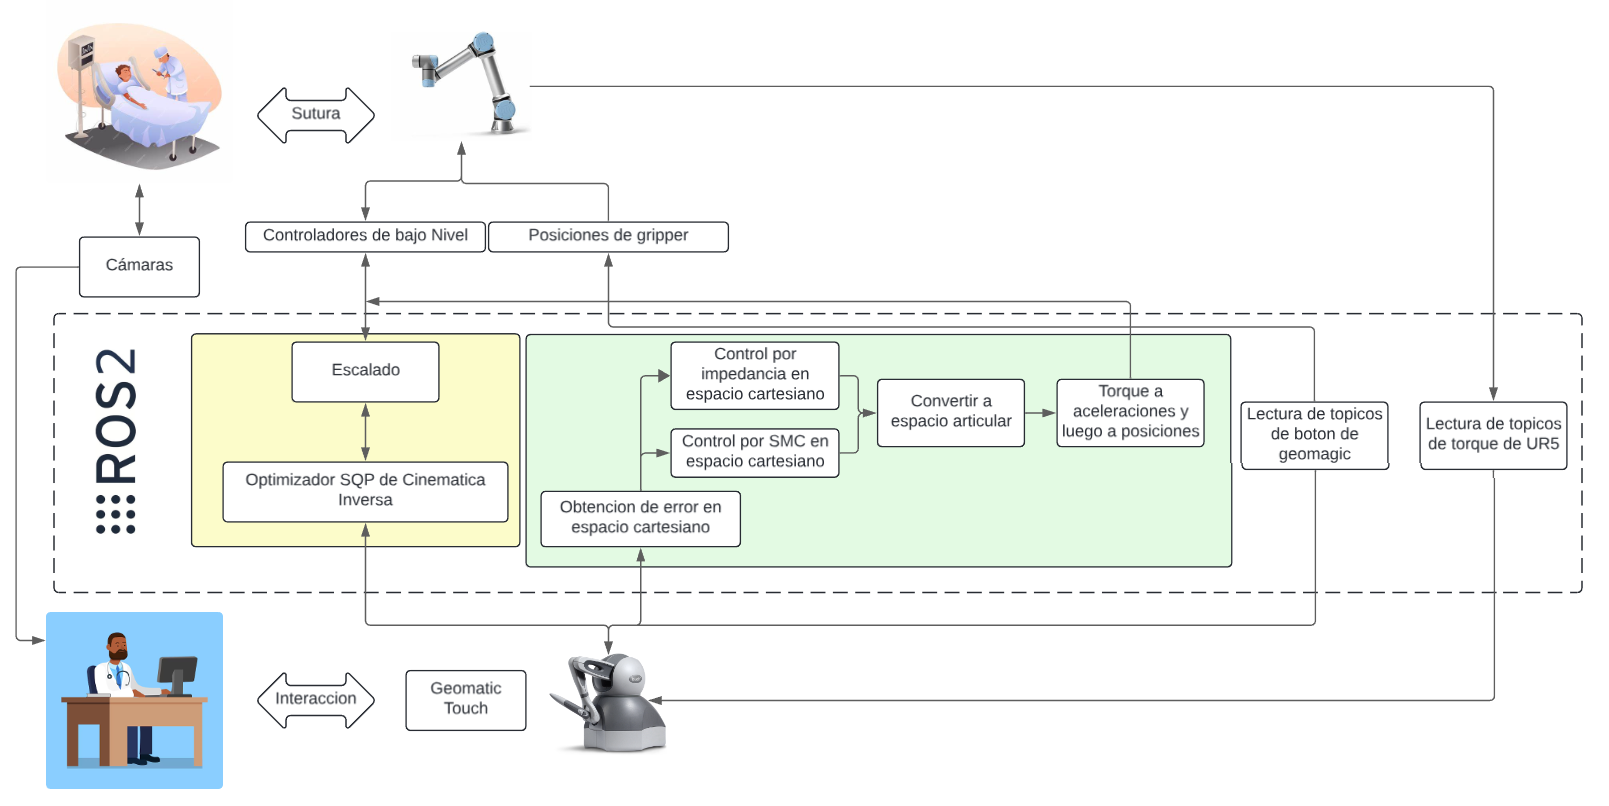
\includegraphics[width=1.0\linewidth]{images/ezquema_teleoperacion.png}
    \caption{Esquema de teleoperación con retroalimentación háptica}
    \label{fig:placeholder}
\end{figure}

\subsection{Control por optimización}

Una de las arquitecturas de control propuestas es un optimizador cuadrático que
permita realizar el proceso de cinemática inversa de manera rápida y precisa.
Se planteó un problema de minimización cuadrática para una función costo que
penaliza el error de pose del efector final, posición y orientación de forma
conjunta, respecto a la velocidad articular, siguiendo restricciones de
velocidad $\boldsymbol{\dot{q}}$ y de valor articular $\boldsymbol{q}$. Para
ello, el error de posición $\boldsymbol{e_p}$ y el de orientación
$\boldsymbol{e_o}$ (representado en su parte vectorial) se agrupan en un único
vector de error de pose $\boldsymbol{e}(q) \in \mathbb{R}^{6}$:

\begin{equation}
    \boldsymbol{e}(q) = \begin{bmatrix} \boldsymbol{e_p} \\ \boldsymbol{e_o} \end{bmatrix}
\end{equation}

y, de manera análoga, el Jacobiano de posición $\boldsymbol{J_p}(q)$ y el de
orientación $\boldsymbol{J_o}(q)$ se apilan en un único Jacobiano geométrico
$\boldsymbol{J}(q) \in \mathbb{R}^{6\times n}$:

\begin{equation}
    \boldsymbol{J}(q) = \begin{bmatrix} \boldsymbol{J_p}(q) \\ \boldsymbol{J_o}(q) \end{bmatrix}
\end{equation}

La importancia relativa entre posición y orientación dentro de la función
costo se incorpora mediante una única matriz de pesos
$\boldsymbol{W}\in\mathbb{R}^{6\times 6}$, construida como una matriz diagonal
por bloques a partir de los vectores escalares $W_p$ y $W_o$, ambos finalmente
fijados en $1.0$ luego de realizar pruebas de sensibilidad y convergencia:

\begin{equation}
    \boldsymbol{W} = \begin{bmatrix} W_p \ & \boldsymbol{0} \\ \boldsymbol{0} & W_o  \end{bmatrix}
\end{equation}

El problema cuadrático resultante se resuelve con el solver OSQP, añadiendo
una regularización de Tikhonov ($\lambda=10^{-6}$) a la Hessiana para
garantizar que sea definida positiva y evitar inestabilidades numéricas cerca
de singularidades del Jacobiano.

\begin{mini*}|s|[0]
    {\boldsymbol{\dot{q}}}{\ensuremath{
        \left\|\boldsymbol{W}\left(\boldsymbol{J}(q)\boldsymbol{\dot{q}}-
        \boldsymbol{e}(q)\right)\right\|^{2}
    }}
    {}
    {\label{eq:minimizationProblemQP}}
\end{mini*}

Luego de operar la función costo general, se pueden ordenar los términos de
manera que despejemos la Matriz Hessiana $\boldsymbol{H}$ y la Matriz Gradiente
$\boldsymbol{\nabla}g(\boldsymbol{q})$, en función del Jacobiano y el error ya
ponderados, $\boldsymbol{J_w}(q)=\boldsymbol{W}\boldsymbol{J}(q)$ y
$\boldsymbol{e_w}(q)=\boldsymbol{W}\boldsymbol{e}(q)$:

\begin{equation}
    \boldsymbol{H}
    = \boldsymbol{J_w(q)}^{T}\boldsymbol{J_w(q)}
    = \boldsymbol{J(q)}^{T}\boldsymbol{W}^{2}\boldsymbol{J(q)}
\end{equation}

\begin{equation}
    \nabla g(\boldsymbol{q})
    = -\boldsymbol{J_w(q)}^{T}\boldsymbol{e_w(q)}
    = -\boldsymbol{J(q)}^{T}\boldsymbol{W}^{2}\boldsymbol{e(q)}
\end{equation}

Finalmente, se definió la función a minimizar de la forma:
\begin{mini*}|s|[0]
    {\boldsymbol{\dot{q}}}{\frac{1}{2}\boldsymbol{\dot{q}}^{T}\boldsymbol{H} +
    \nabla g(\boldsymbol{q})\boldsymbol{\dot{q}}}
    {\label{eq:minimizationProblem}}
    {}
\end{mini*}
\begin{equation*}
    |\boldsymbol{\Delta q}| < 0.5 \text{ rad por iteración}
\end{equation*}
\begin{equation*}
    |\boldsymbol{q}|<2\pi
\end{equation*}

El resultado es un valor de paso $\boldsymbol{\Delta q}$ acotado directamente a
un máximo de $0.5$ rad por iteración; cuando el valor articular resultante se
acerca al límite físico de $\pm 2\pi$, la cota se reduce al margen restante
disponible hasta dicho límite, de modo que el paso nunca produce una
configuración articular fuera de rango. Este valor de paso se adiciona a la
configuración articular real del robot para ser enviado en la siguiente
iteración del bucle del programa principal.

\begin{equation}
    \boldsymbol{q}_{k+1} = \boldsymbol{q}_k + \boldsymbol{\Delta q}
\end{equation}

\subsection{Control por modo deslizante}

La implementación del controlador SMC sigue la ley de control descrita en el
capítulo de marco teórico: en cada ciclo de control se calcula la superficie
de deslizamiento $\boldsymbol{S}$ a partir del error de seguimiento cartesiano
y sus derivadas, y se obtiene el torque de control $\boldsymbol{\tau}$
correspondiente. Las ganancias $\boldsymbol{\lambda}$, $\boldsymbol{k}$ y
$\boldsymbol{k_2}$ son vectores de 6 componentes, una por cada eje del error
cartesiano (posición y orientación), aplicadas mediante producto elemento a
elemento ($\boldsymbol{\lambda}\odot\boldsymbol{e}$); esto es matemáticamente
equivalente a aplicar cada ganancia como la diagonal de una matriz
($\text{diag}(\boldsymbol{\lambda})\cdot\boldsymbol{e}$), forma en la que se
presentan en el capítulo de marco teórico. Únicamente $k_3$ se mantiene como
una ganancia escalar única que controla la pendiente de la función $\tanh$
que suaviza la ley de control. Los valores utilizados se
muestran en la Tabla \ref{tab:ganancias_smc}.

\begin{table}[H]
    \centering
    \begin{tabular}{c|c}
        $\boldsymbol{\lambda}$ & $20,20,20,20,20,20$ \\
        $\boldsymbol{k}$       & $50,50,50,50,50,50$ \\
        $\boldsymbol{k_2}$     & $10,10,10,10,10,10$ \\
        $k_3$                  & $10$
    \end{tabular}
    \caption{Ganancias del control por modo deslizante}
    \label{tab:ganancias_smc}
\end{table}

Para evitar inestabilidades numéricas al acercarse a configuraciones
singulares del Jacobiano, la ley de control emplea una pseudo-inversa
amortiguada:
\begin{equation}
    \boldsymbol{J}^{\dagger} = \boldsymbol{J}^T \left(
    \boldsymbol{J}\boldsymbol{J}^T + \delta^2 \boldsymbol{I} \right)^{-1}
\end{equation}
donde $\delta$ es un factor de amortiguamiento pequeño.

\subsection{Control por impedancia}

La implementación del controlador por impedancia sigue la ley de torque
computado descrita en el capítulo de marco teórico: en cada ciclo de control
se calcula el error de pose $\boldsymbol{e}$ y su derivada respecto a la
trayectoria deseada, y se proyecta la dinámica virtual
masa-resorte-amortiguador
al espacio articular mediante el Jacobiano del robot. Las ganancias
$\boldsymbol{K_d}$
(rigidez) y $\boldsymbol{D_d}$ (amortiguamiento) son igualmente vectores de 6
componentes, aplicados como la diagonal de una matriz
($\text{diag}(\boldsymbol{K_d})\cdot\boldsymbol{e}$), organizados según el
formato $K_x, K_y, K_z, K_{\phi x}, K_{\phi y}, K_{\phi z}$. Para esta
arquitectura se emplearon los valores mostrados en la Tabla
\ref{tab:ganancias_impedancia}.

\begin{table}[H]
    \centering
    \begin{tabular}{c|c}
        $\boldsymbol{K_d}$ & $1850,1850,1850,500,500,500$ \\
        $\boldsymbol{D_d}$ & $10,10,10,10,10,10$
    \end{tabular}
    \caption{Ganancias del control por impedancia}
    \label{tab:ganancias_impedancia}
\end{table}

\subsection{Frecuencia de control y conversión de torque a posición}

Dado que las restricciones del fabricante impiden comandar al UR5 directamente
mediante señales de torque, la salida $\boldsymbol{\tau}$ de ambos
controladores dinámicos (SMC e impedancia) se convierte a una referencia de
posición articular antes de ser transmitida al robot. Los registros de los
ensayos muestran que, en la práctica, el controlador QP operó cerca de los
$500$ Hz nominales ($dt\approx2.0$ ms), mientras que SMC e impedancia
operaron efectivamente en un rango de $100$--$120$ Hz ($dt\approx8$--$9$ ms),
por debajo de los $500$ Hz configurados como frecuencia objetivo.

Para el controlador por impedancia, la conversión se realiza mediante un
esquema de Euler semi-implícito: primero se actualiza la velocidad articular
con la aceleración calculada,
$\boldsymbol{\dot{q}}_{k+1}=\boldsymbol{\dot{q}}_k+\boldsymbol{\ddot{q}}\,dt$,
y luego la posición con la velocidad ya actualizada,
$\boldsymbol{q}_{k+1}=\boldsymbol{q}_k+\boldsymbol{\dot{q}}_{k+1}\,dt$. Para el
controlador SMC, en cambio, se emplea una expansión de segundo orden (modelo
de aceleración constante):
\begin{equation}
    \boldsymbol{q}_{k+1} = \boldsymbol{q}_k + \boldsymbol{\dot{q}}_k \, dt +
    \frac{1}{2}\boldsymbol{\ddot{q}} \, dt^2
\end{equation}
Este segundo esquema tiene un error de truncamiento local de orden
$O(dt^3)$, frente a $O(dt^2)$ del esquema semi-implícito, por lo que resulta
más preciso en este contexto de lazo cerrado, donde la velocidad articular se
vuelve a medir directamente del robot en cada ciclo en lugar de acumularse
por integración abierta durante muchos pasos.

\section{Interfaz de lanzador}
\label{sec:interfaz_lanzador}

El lenguaje de programación usado para los bucles de control y la
transmisión/recepción de datos del robot es C++, lenguaje en el que se
definieron clases para cada nodo usado. La arquitectura de gestión de paquetes
y ejecutables fue ROS2 Humble, lo que permitió la comunicación entre los
distintos programas desarrollados gracias a su sistema de nodos publicadores y
suscriptores. Si bien los programas y nodos se pueden lanzar desde la terminal
o desde un ejecutable, parte de los objetivos de este trabajo de investigación
es la integración de todo el sistema en un solo entorno, capaz de ser
reproducible y facilitando la ejecución de los nodos dentro de la arquitectura
ROS. Bajo esta premisa se desarrolló una interfaz de usuario basada en el
framework Qt5 y usando Python (PyQt5) como el lenguaje de programación
encargado de la lógica de funcionamiento.

La interfaz de usuario integra los lanzadores/driver del sistema, que permite
conectar mediante red (ethernet o wifi) el equipo con los dos robots, y
mediante usb a los periféricos, como son los dispositivos hápticos, la cámara y
los puertos ModBus para los grippers.
\subsection{Lógica en C++}
El control y la lógica de funcionamiento de cada esquema de control se
trabajaron en nodos de ROS desarrollados en C++, esto debido a la necesidad de
reducir los tiempos de ejecución que se requieren en el bucle principal de
control. Se dividió la lógica interna de cada controlador en nodos que al ser
compilados generan librerías internas que pueden ser usadas por distintos nodos
dentro del espacio de trabajo, reduciendo la carga computacional al no
necesitar la carga de variables o funciones extras. Por otro lado, cada nodo se
desarrolló para poder admitir argumentos y un espacio de trabajo independiente,
por lo que se pudo usar el mismo nodo para los dos robots del banco de trabajo
sin problemas.

\subsection{Interfaz en Python}

La interfaz que carga cada uno de los nodos y lanzadores se desarrolló con
PyQt5
con el objetivo de integrar la herramienta gráfica RViz, diseñada bajo la
arquitectura Qt5 y compatible con interfaces desarrollada en esta. El diseño de
la interfaz está orientada a poder configurar tanto el robot como el modo de
operación.

\begin{figure}[H]
    \centering
    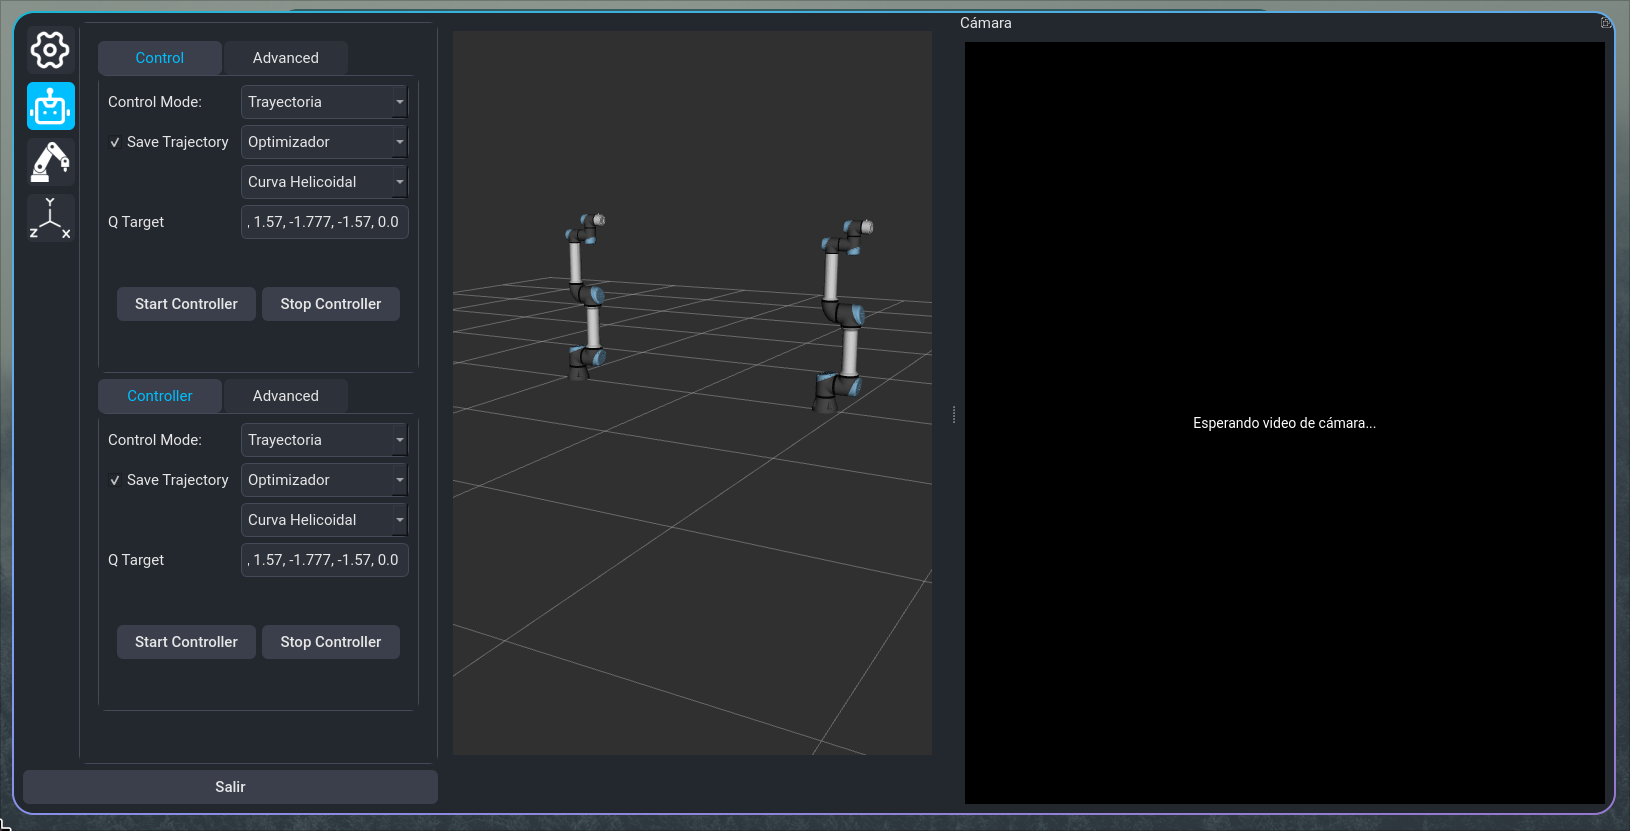
\includegraphics[width=1\linewidth]{images/interfaz.png}
    \caption{Interfaz en PyQt5. Se muestran de izquierda a derecha el área de
        configuración, el visualizador 3D de Rviz y el visualizador de la
        cámara}
    \label{fig:placeholder}
\end{figure}

\section{Diseño y fabricación de adaptadores}

\subsection{Adaptador de una pinza genérica para el gripper Robotiq 2F‑85 para
    UR5}

El diseño de las piezas se realizó utilizando el software Fusion 360 de la
empresa Autodesk. Asimismo, se utilizó instrumentos de precisión de 0.01
milímetros para la medición de los elementos físicos que se buscan adaptar.
Estas piezas 3D fueron impresas con PLA al 50\% de densidad en el laboratorio
de
mecatrónica 201 de la UTEC.

\begin{figure}[H]
    \centering

    \begin{minipage}{0.8\textwidth}
        \centering
        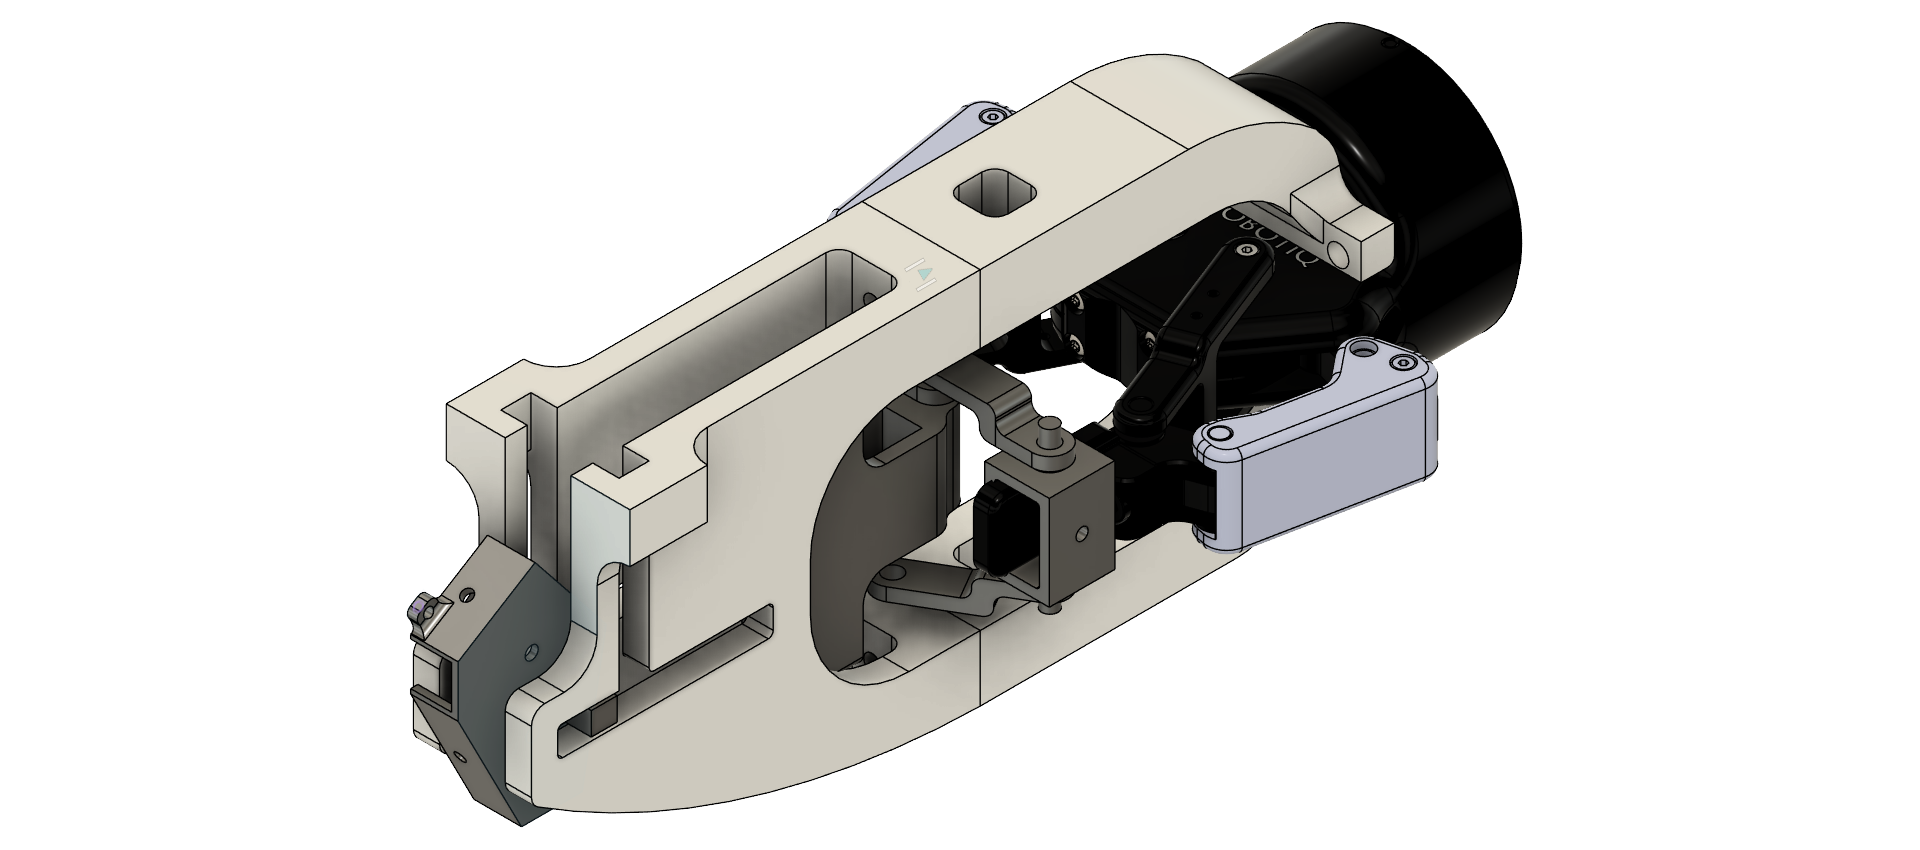
\includegraphics[width=\linewidth]{images/ensamble_try3 v11.png}
        \caption*{(a)  Ensamblaje final gripper 2f 85 de la empresa Robotiq}
    \end{minipage}
    \hfill
    \begin{minipage}{0.8\textwidth}
        \centering
        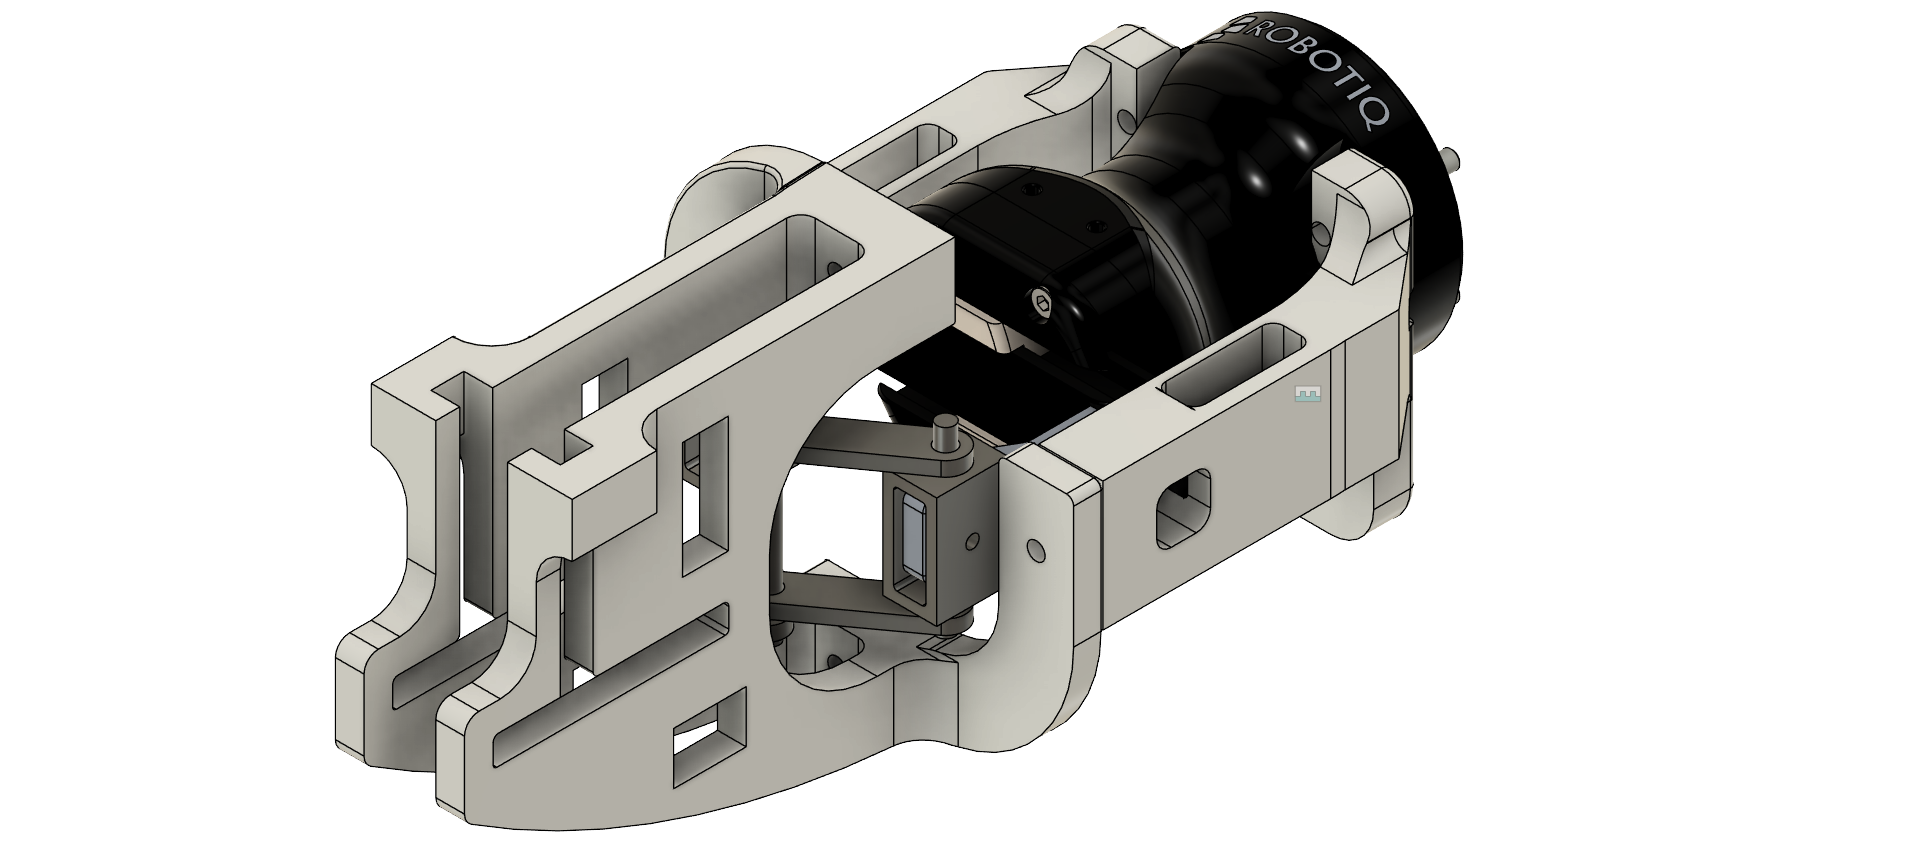
\includegraphics[width=\linewidth]{images/handegripp v6.png}
        \caption*{(b) Ensamblaje final gripper hand-e de la empresa Robotiq}
    \end{minipage}
    \caption{Vistas principales del ensamble final.}
    \label{fig:vistas_pinza_ensamble}
\end{figure}

\subsection{Adaptador del efector final del Geomagic Touch para sutura}

El dispositivo háptico cuenta con una adaptación específica para el
procedimiento de sutura, ya que este proceso requiere la sujeción de una aguja
e hilo. Dado que el Geomagic Touch se puede desacoplar, se diseñó un adaptador
en forma de lápiz que se acopla al efector final para desempeñar esta función.
Este diseño se basa en un mecanismo similar al presentado en
\cite{arm_pivot_joints_stiffness}, donde se logró adaptar un sistema que
permite la inserción de los dedos para evaluar el efecto de un punto pivote
sobre la rigidez que se mide.

\begin{figure}[H]
    \centering

    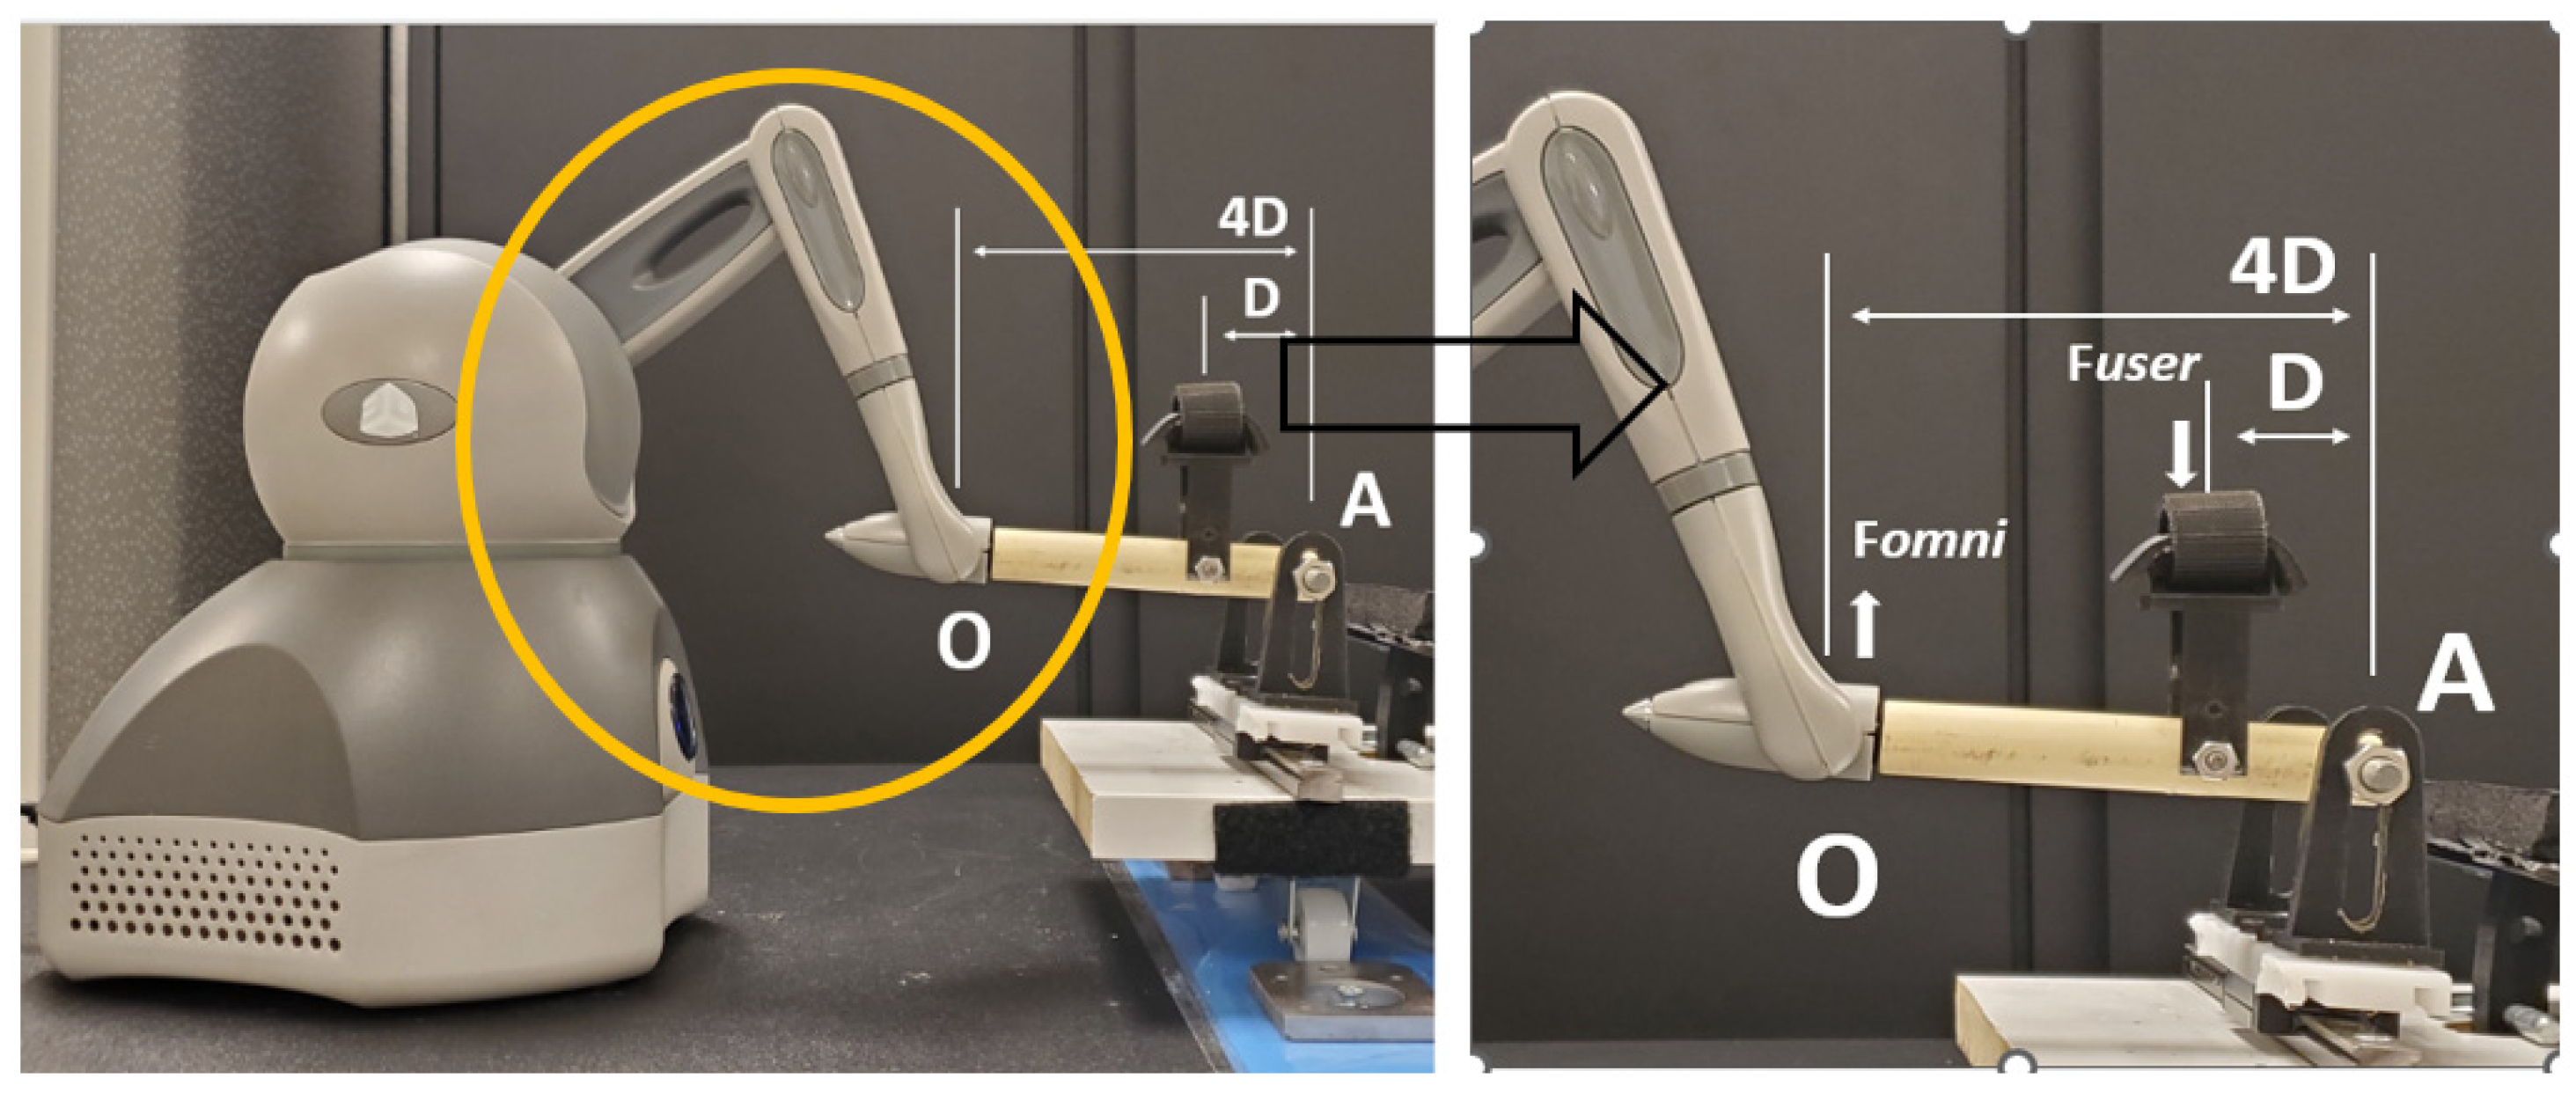
\includegraphics[width=0.75\linewidth]{images/geomagic_adaptation_example.png}
    \caption{Modificación al efector final del módulo geomagic touch en
        \cite{arm_pivot_joints_stiffness}}
    \label{fig:geomagic_adaptation_example}
\end{figure}

\section{Validación experimental}

La validación experimental se organizó en tres etapas. En la primera, se
comparó el desempeño de las tres arquitecturas de control (impedancia, modo
deslizante y optimización cuadrática) mediante pruebas de seguimiento a
trayectoria en simulación, evaluando cada arquitectura sobre dos trayectorias
de referencia de dificultad creciente: una trayectoria recta y una curva
helicoidal de radio variable, esta última pensada para exigir un seguimiento
más demandante en aceleración y cambio de dirección. Durante el desarrollo se
exploró también una trayectoria circular de radio constante, intermedia en
dificultad entre ambas, aunque finalmente no formó parte de las corridas
reportadas en el capítulo de Resultados. En la segunda etapa, se validó el
sistema completo mediante un movimiento de teleoperación guiado por el
operador a través del Geomagic Touch, empleando la arquitectura de mejor
desempeño identificada en la primera etapa. Finalmente, en la tercera etapa
se evaluó el sistema integrado (teleoperación, control y hardware) ejecutando
una sutura sobre un kit de entrenamiento de cirugía laparoscópica.

\subsection{Pruebas de seguimiento a trayectoria}

Para cada una de las seis combinaciones evaluadas (3 arquitecturas $\times$ 2
trayectorias) se registraron: el seguimiento tridimensional del efector final
respecto a la trayectoria de referencia, el error de seguimiento en cada eje
cartesiano ($x$, $y$, $z$), y el esfuerzo de control requerido por cada
arquitectura. La ecuación de la trayectoria recta se detalla en el capítulo de
Resultados. La curva helicoidal, cuya amplitud crece de forma exponencial
desde el punto inicial hasta un radio máximo $A$ con constante de tiempo
$1/c_0$, se define como:

\begin{equation}
    \begin{cases}
        x(t) = x_0 + A_x\left(1-e^{-c_0 t}\right)\sin(\omega_n t) \\
        y(t) = y_0 + A_y\left(1-e^{-c_0 t}\right)\cos(\omega_n t) \\
        z(t) = z_0 + A_z\left(1-e^{-c_0 t}\right)\sin(\omega_n t)
    \end{cases}
\end{equation}

% Pendiente: reportar los valores numéricos de A_x/A_y/A_z, omega_n, c0 usados
% en las corridas finales (la duración de cada prueba se puede tomar de los
% registros CSV: linea recta ~63s IMP / ~51s SMC / ~26s QP; curva helicoidal
% ~122s IMP / ~140s SMC / ~38s QP).

\subsection{Validación de teleoperación}

Con la arquitectura de mejor desempeño identificada en las pruebas de
seguimiento, se validó el sistema completo mediante un ejercicio de
teleoperación en el que el operador guio el efector final del UR5 a través del
Geomagic Touch, registrando el seguimiento del robot respecto al movimiento
comandado por el operador en los tres ejes cartesianos.
% Pendiente: describir el protocolo exacto de esta prueba (duración, tarea
% realizada, criterio de éxito).

\subsection{Validación con el banco de trabajo}

Finalmente, se evaluó el sistema integrado (teleoperación, control y
hardware) ejecutando una sutura sobre un kit de entrenamiento de cirugía
laparoscópica, registrando el tiempo de finalización de la tarea y el error
máximo de seguimiento durante su ejecución.
% Pendiente: describir el protocolo completo (número de repeticiones,
% criterio de éxito) y reportar aquí las métricas que hoy solo aparecen en
% las Conclusiones (tiempo medio de sutura, error máximo de seguimiento,
% episodios de Jacobiano indeterminado), de modo que no sean la primera vez
% que el lector las ve.